\documentclass[a4paper,10pt]{article}
\usepackage[utf8]{inputenc}
\usepackage{graphicx}
\usepackage{amsmath}
\usepackage{graphicx,natbib}%amssymb

%opening
\title{}
\author{}

\begin{document}

\maketitle

% \begin{abstract}
% 
% \end{abstract}

\section{Data and Results}

The population consists of children in elementary school attending 2nd, 4th and 6th grade. The game was played in couples of children of the same gender. 18 couples (9 female) from 2nd grade, 27 couples (13 female) from 4th grade and 15 couples (10 female) from 6th grade. On average, 2nd graders completed 6.3 trials, 4th graders completed 12.2 trials and 6th graders 17 trials of the game. Without removing the first trials, the fraction of ``success'' trials was 0.14, 0.57  and 0.77 for each grade
respectively. The histograms of the performance are shown in figure \ref{fig:histo_performance}


% \begin{equation}
%     \label{simple_equation}
%     \alpha = \sqrt{ \beta }
% \end{equation}



\begin{figure}
    \centering
    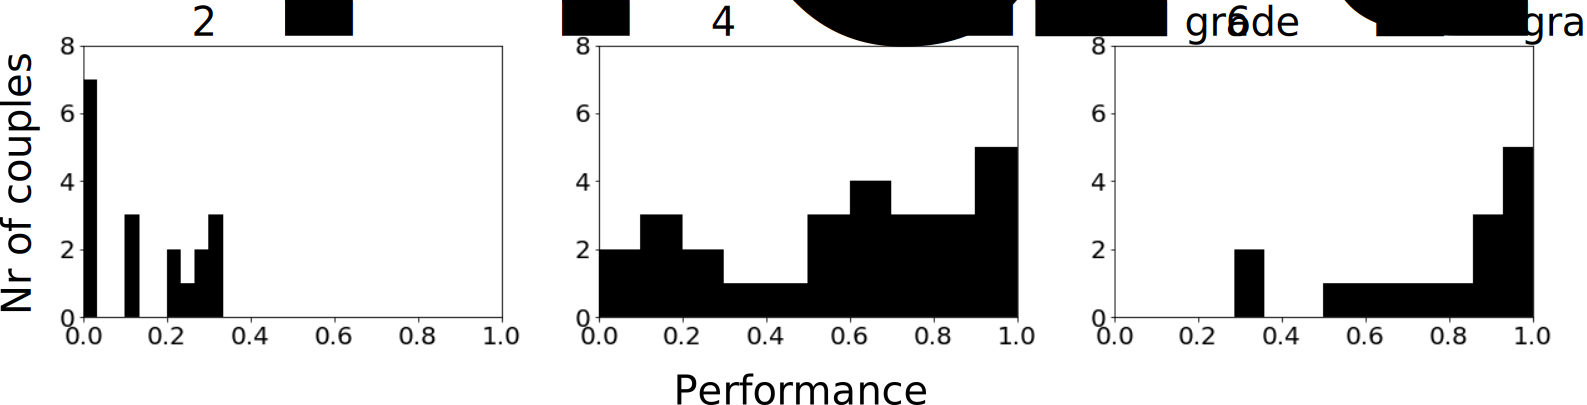
\includegraphics[width=6.0in]{figures/performance_histograms.pdf}
    \caption{Performance (fraction of rectangles found) distributions for each grade.}
    \label{simulationfigure}
\end{figure}


%\begin{figure}
%    \centering
%    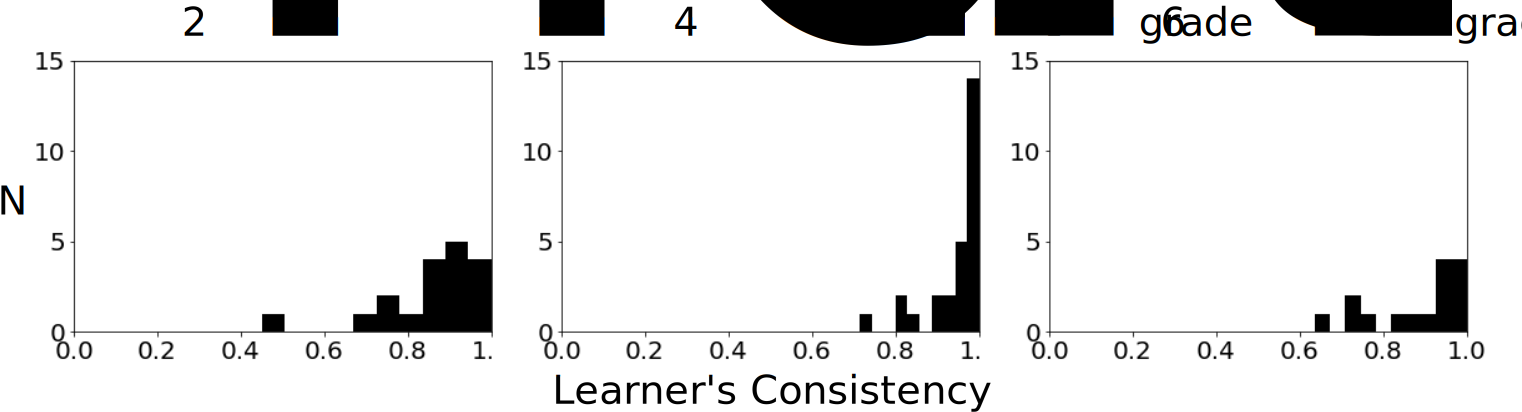
\includegraphics[width=6.0in]{figures/learners_consistency.pdf}
%    \caption{Consistency of the learners. Inconsistent learner's inferences are those in which the drawn rectangle contains a cross sample inside or leaves a circle sample outside.}
%    \label{simulationfigure}
%\end{figure}


\begin{figure}
    \centering
    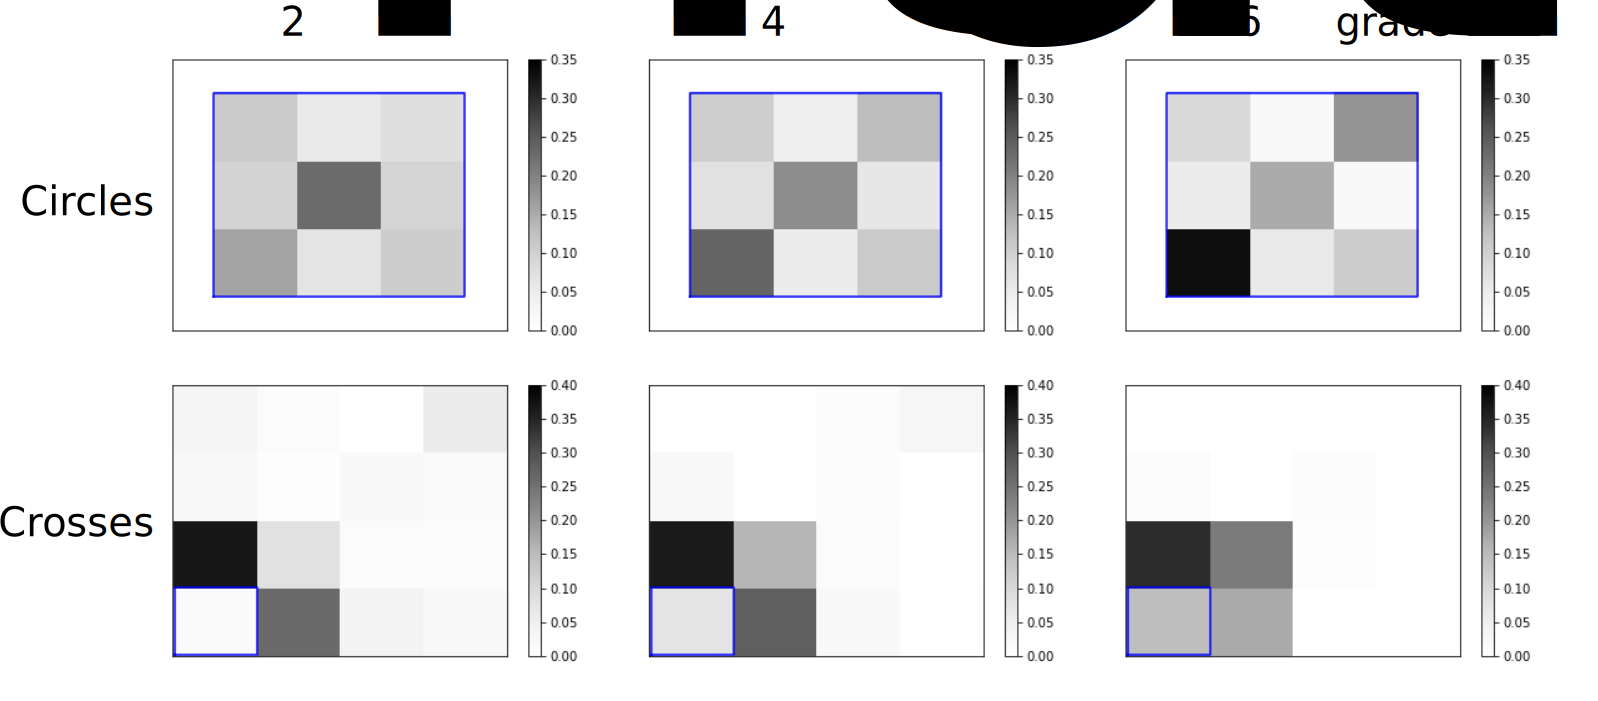
\includegraphics[width=6.0in]{figures/samples_positions_histograms.pdf}
    \caption{Position of the examples relative to the rectangle that the teacher saw. The histograms are averaged across couples for each grade.}
    \label{simulationfigure}
\end{figure}

\begin{figure}
    \centering
    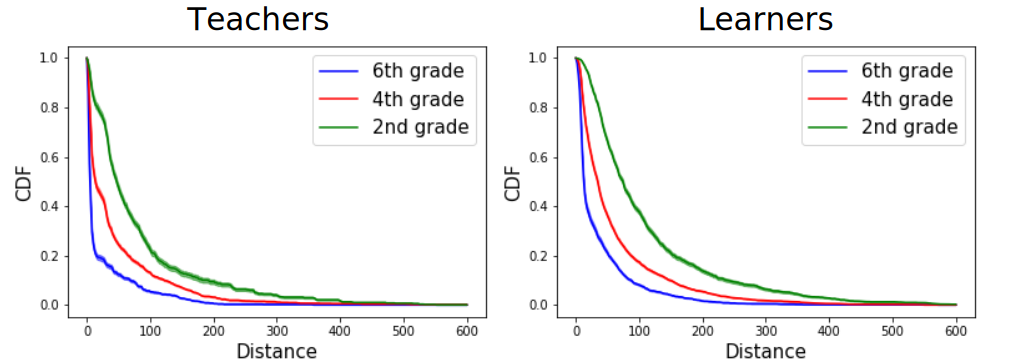
\includegraphics[width=6.0in]{figures/Distance_to_corners_teachers_learners.pdf}
    \caption{Cumulative distribution function of the distances of the selected samples with respect to the closest corner of the rectangle. The left plot shows the distances of the examples with respect to the rectangle seen by the teacher. The right plor shows the distance with respect to the rectangle drawn by the learner. The CDF for each population (2nd, 4th and 6th grade) was averaged across subjects and the shaded area denotes standard error bars.}
    \label{dist_2_corners}
\end{figure}


\subsection{The Model}

We implemented the model presented by Shafto et all:

\begin{align}
 P_T (d|h) = \frac{P_L (h|d) P_T0(h)}{P_T(h)} \\
 P_L (h|d) = \frac{P_T (d|h) P_L0(d)}{P_L(d)} \notag
\end{align}

The implementation works as follows. 

\begin{itemize}
 \item Build a binary matrix M of size $E x H$ where E is the number of possible examples to be selected by the teacher and $H$ is the number of possible hypothesis (rectangles). The element $m_{e,h}$ equals 1 if the example $e$ is compatible with the hypothesis $h$ and zero otherwise.
 \item Normalize M column wise to get a matrix $T$
 \item Normalize T row wise to get a matrix $L$
 \item Normalize L colum wise to update $T$
 \item Repeat until T and L converge.
\end{itemize}

After convergence the elements $t_{e,h}$ of matrix $T$ represents the probability $P_T(e|h)$. Conversely $l_{e,h}$ represents $P_L(h|e)$. We performed this iterative process at each move (selected example by the teacher and guessed rectangle by the learner) to yield a model prediction for the next example and guess.


\begin{figure}
    \centering
    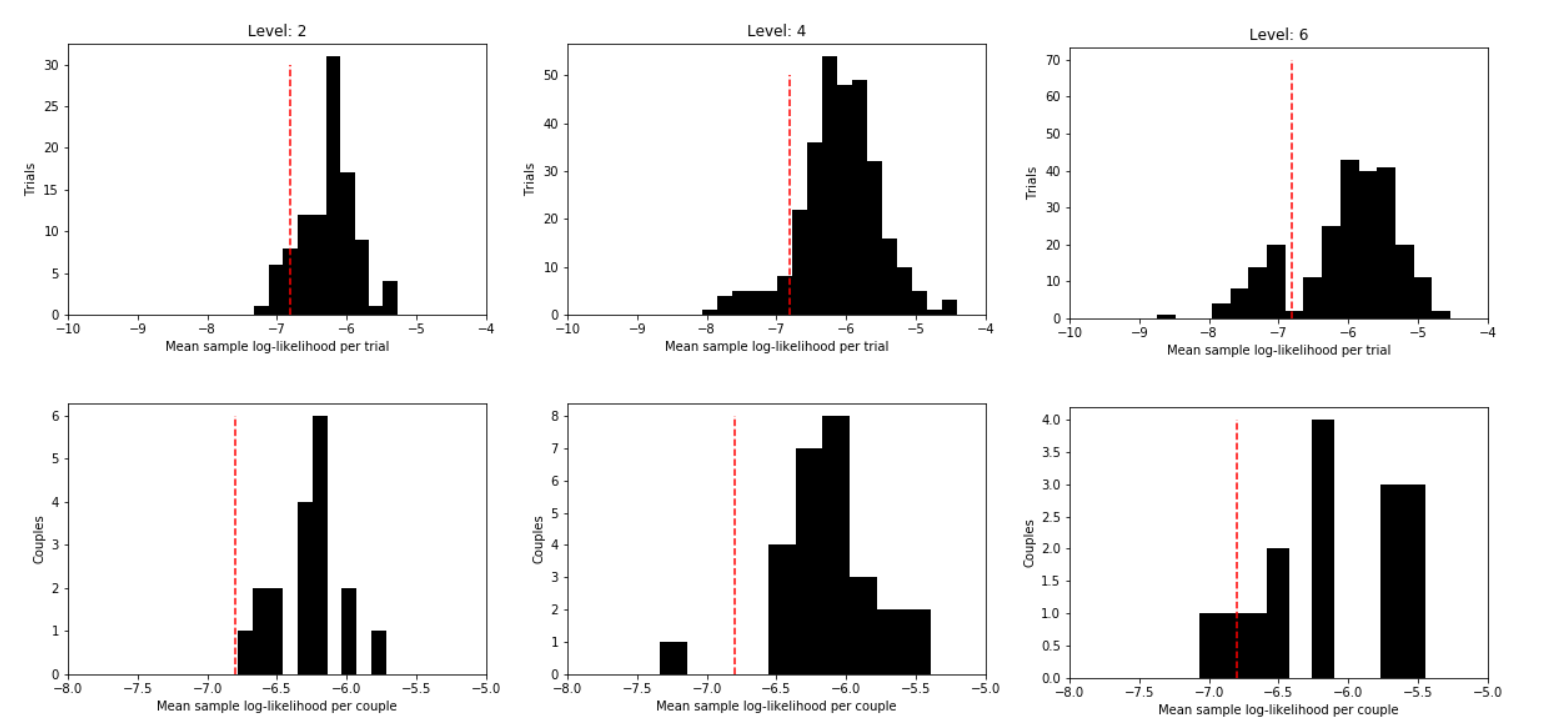
\includegraphics[width=6.0in]{figures/likelihood_of_samples.pdf}
    \caption{Mean likelihood per selected example $P(s|h)$ for each trial (top row), and averaged across trials (bottom row). Red vertical line shows the expected likelihood given a uniform distribution of $P(s|h)$.}
    \label{dist_2_corners}
\end{figure}

\begin{figure}
    \centering
    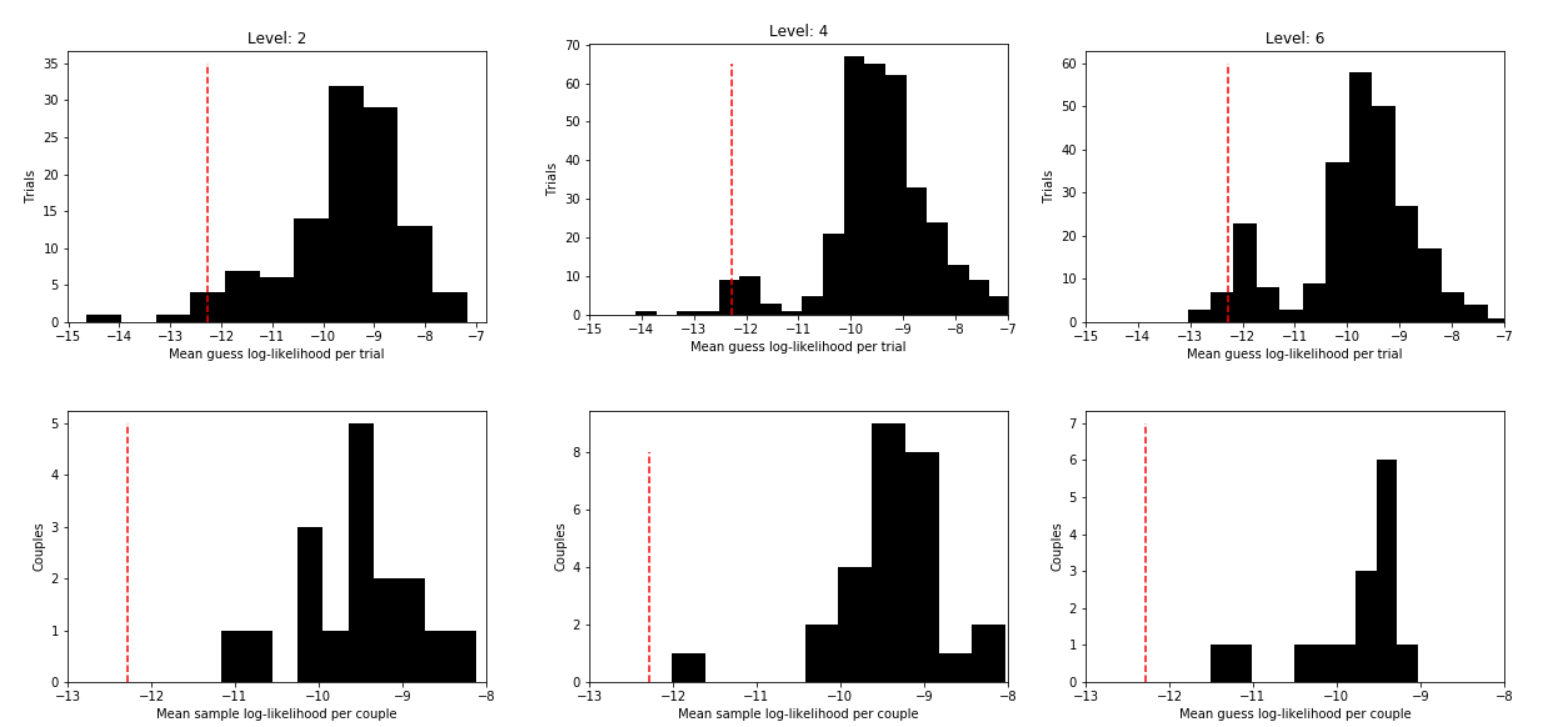
\includegraphics[width=6.0in]{figures/likelihood_of_guesses.pdf}
    \caption{Mean likelihood per guess $P(h|s)$ for each trial (top row), and averaged across trials (bottom row). Red vertical line shows the expected likelihood given a uniform distribution of $P(h|s)$.}
    \label{dist_2_corners}
\end{figure}


\begin{figure}
    \centering
    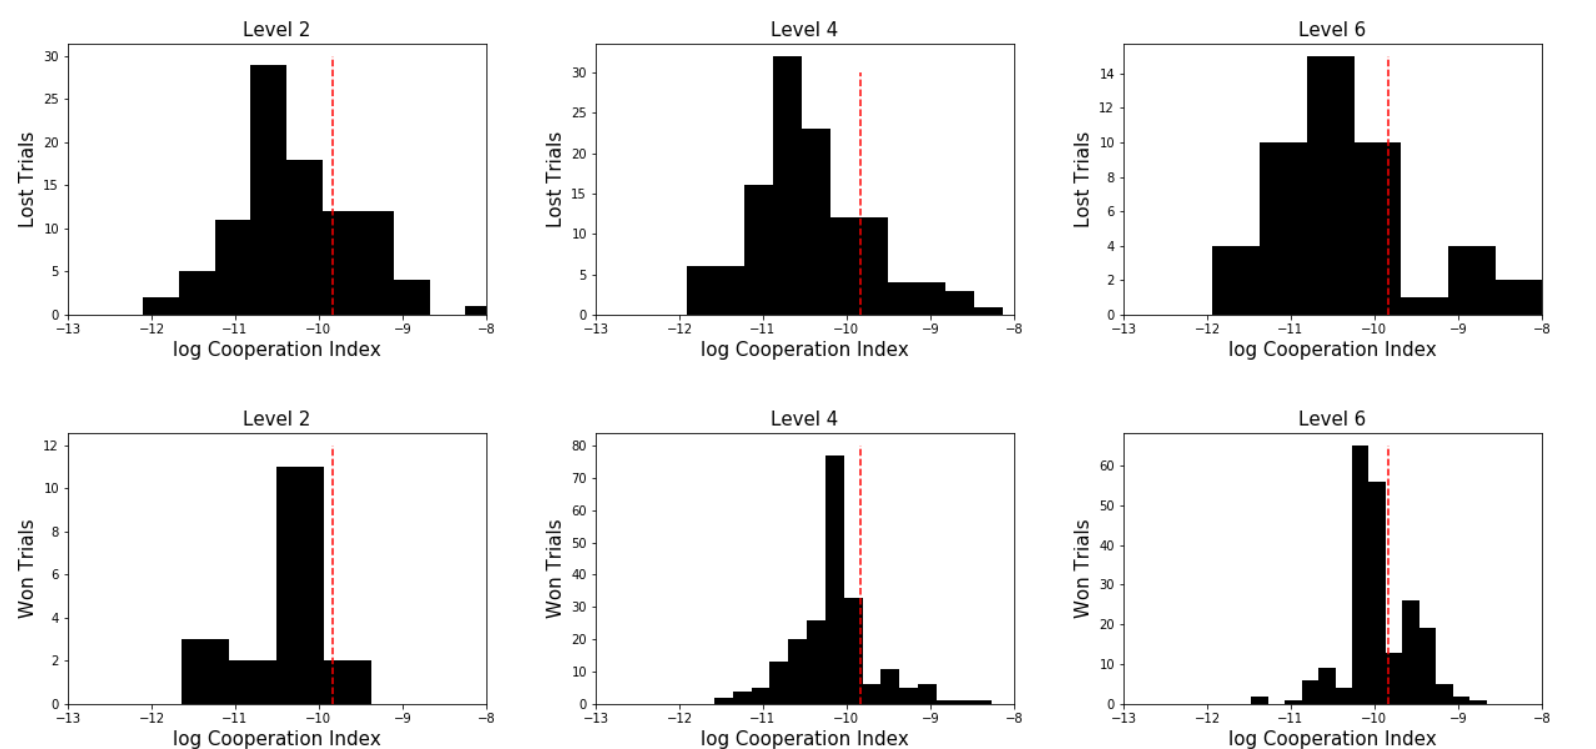
\includegraphics[width=6.0in]{figures/Cooperation_Index.pdf}
    \caption{Cooperation index computed at the end of each trial. Top row shows the successfull trials and the bottom row shows the unseccessfull ones. The red vertical line shows the initial value of CI (before any examples were given).}
    \label{dist_2_corners}
\end{figure}



\begin{figure}
    \centering
    \includegraphics[width=6.0in]{figures/high_likelihood_per_sample.pdf}
    \caption{Example of a trial with high agreement between the model prediction of samples to be selected and the teacher's behavior, i.e. high likelihood per sample.}
    \label{}
\end{figure}

\begin{figure}
    \centering
    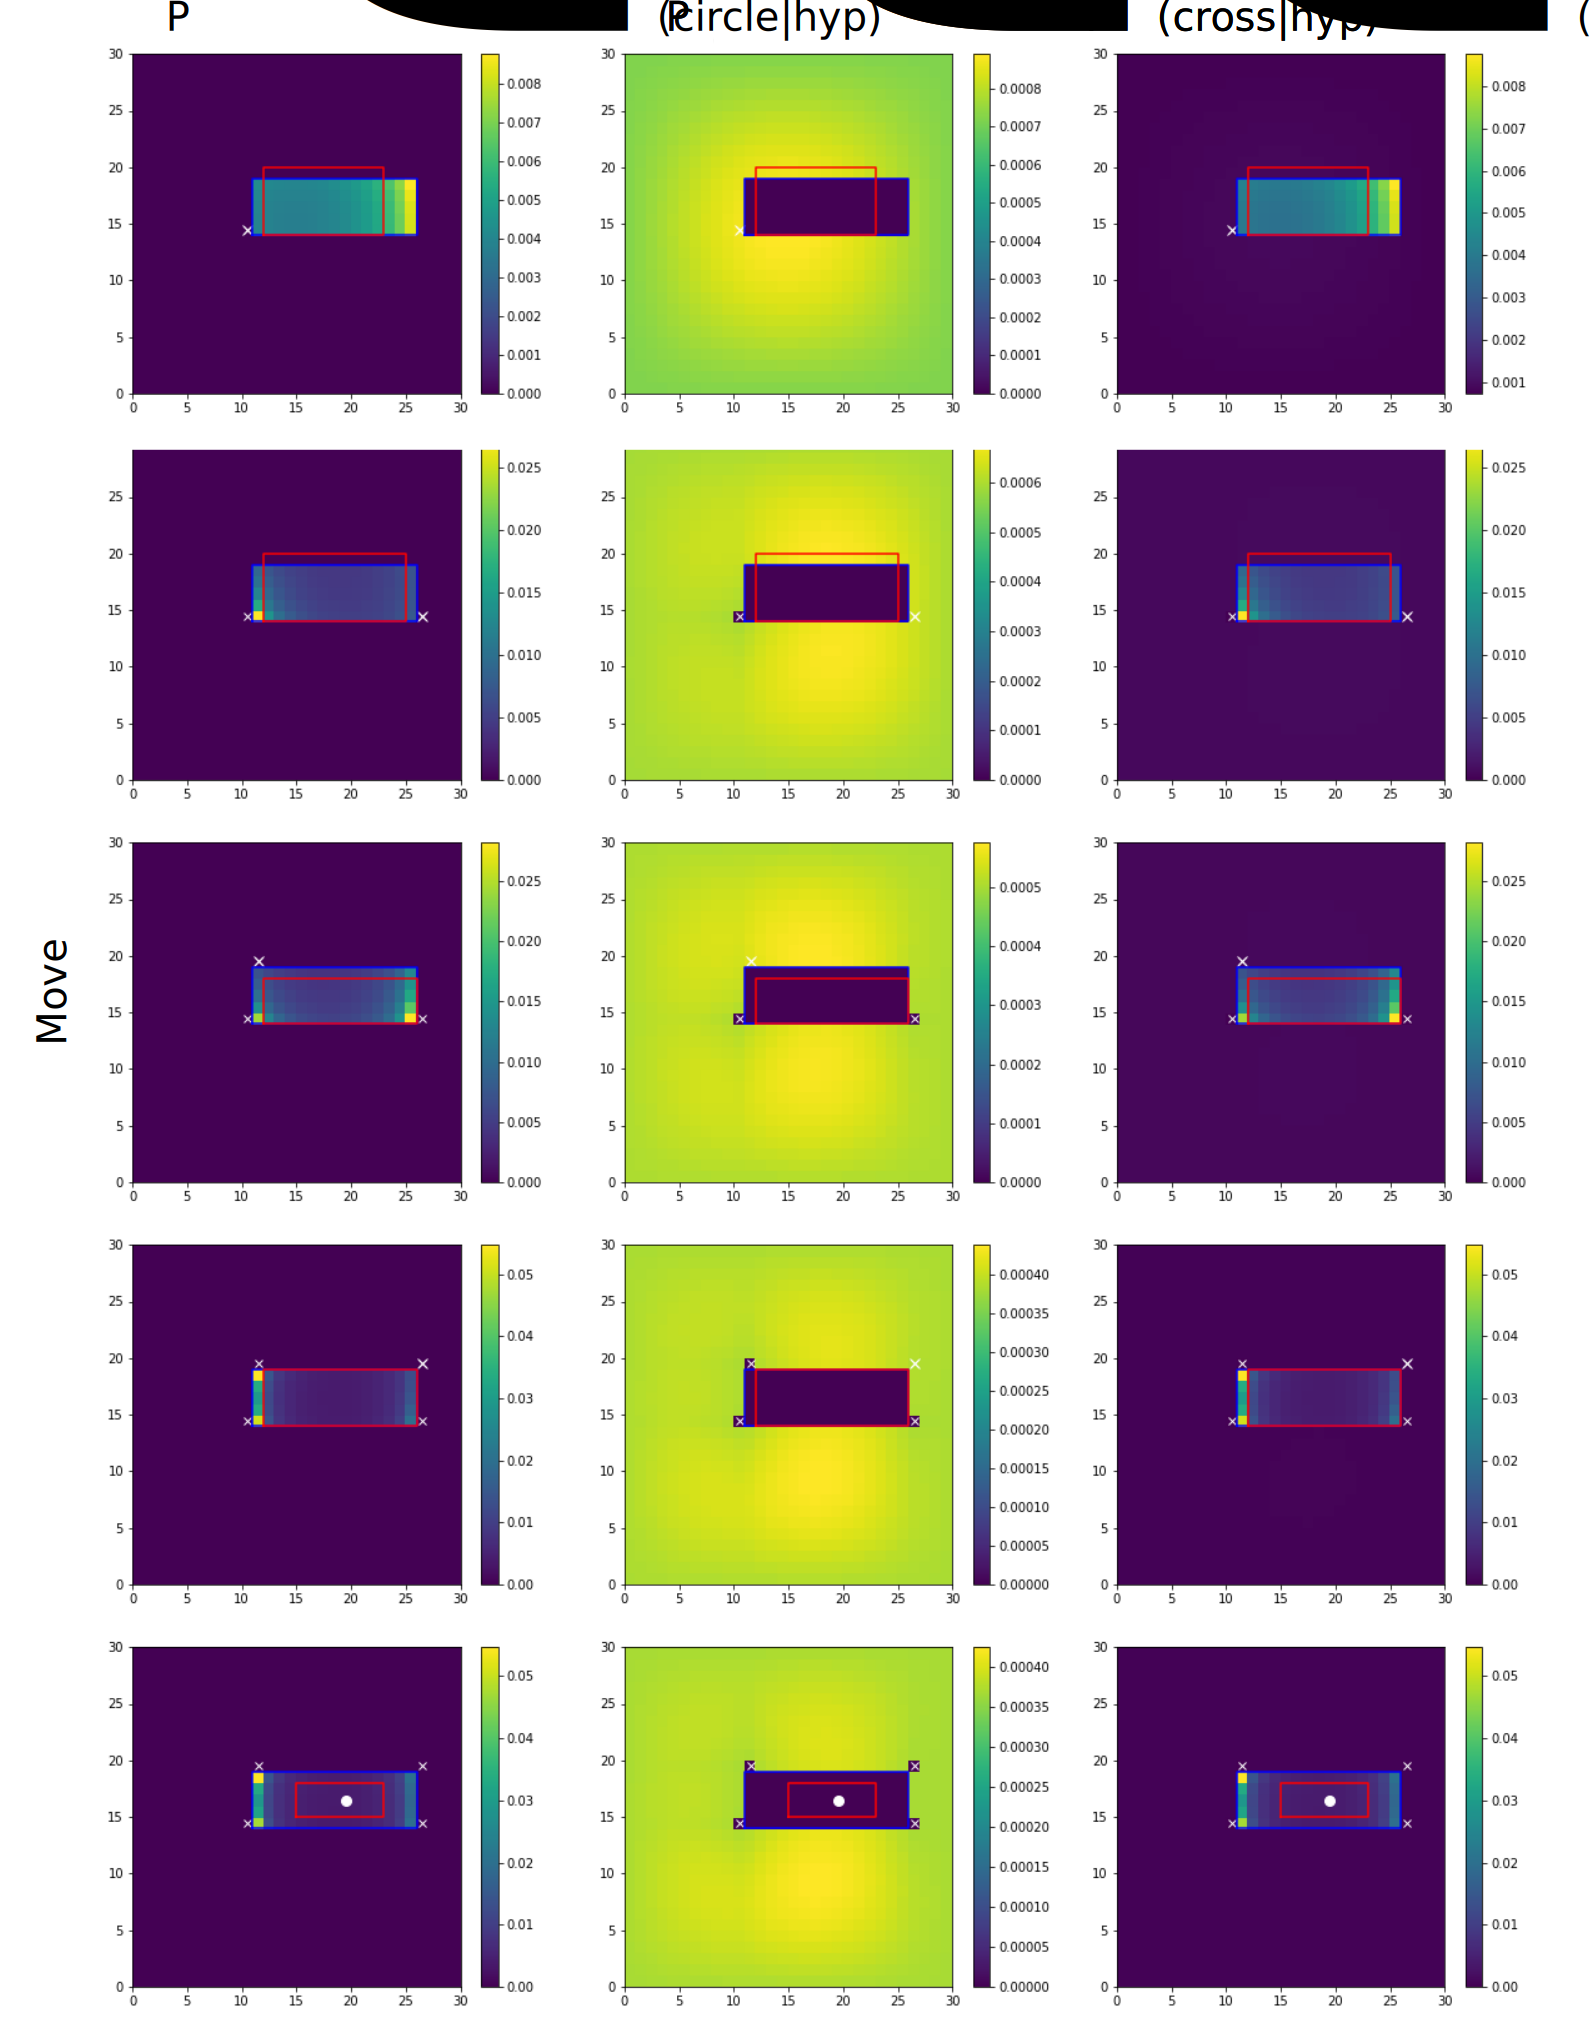
\includegraphics[width=6.0in]{figures/low_likelihood_per_sample.pdf}
    \caption{Example of a trial with LOW agreement between the model prediction of samples to be selected and the teacher's behavior, i.e. low likelihood per sample.}
    \label{}
\end{figure}





\end{document}




